\chapter{Sterownik}

Aby zrealizować zamierzony cel, wybrana została technologia zbliżeniowa RFID, gdyż jest ona obecnie bardzo popularna i można znaleźć wiele sprzętu w niej operujących.

\section{Wykorzystany sprzęt}

Jako system bazowy został wykorzystany Raspberry Pi w wersji 2 B v1.1 (Rysunek \ref{fig:raspberry}). Różni się on od poprzednich wersji płytki ilością pinów oraz wielkością pamięci operacyjnej i szybszym mikroprocesorem.

\begin{figure}[h!]
	\centering
	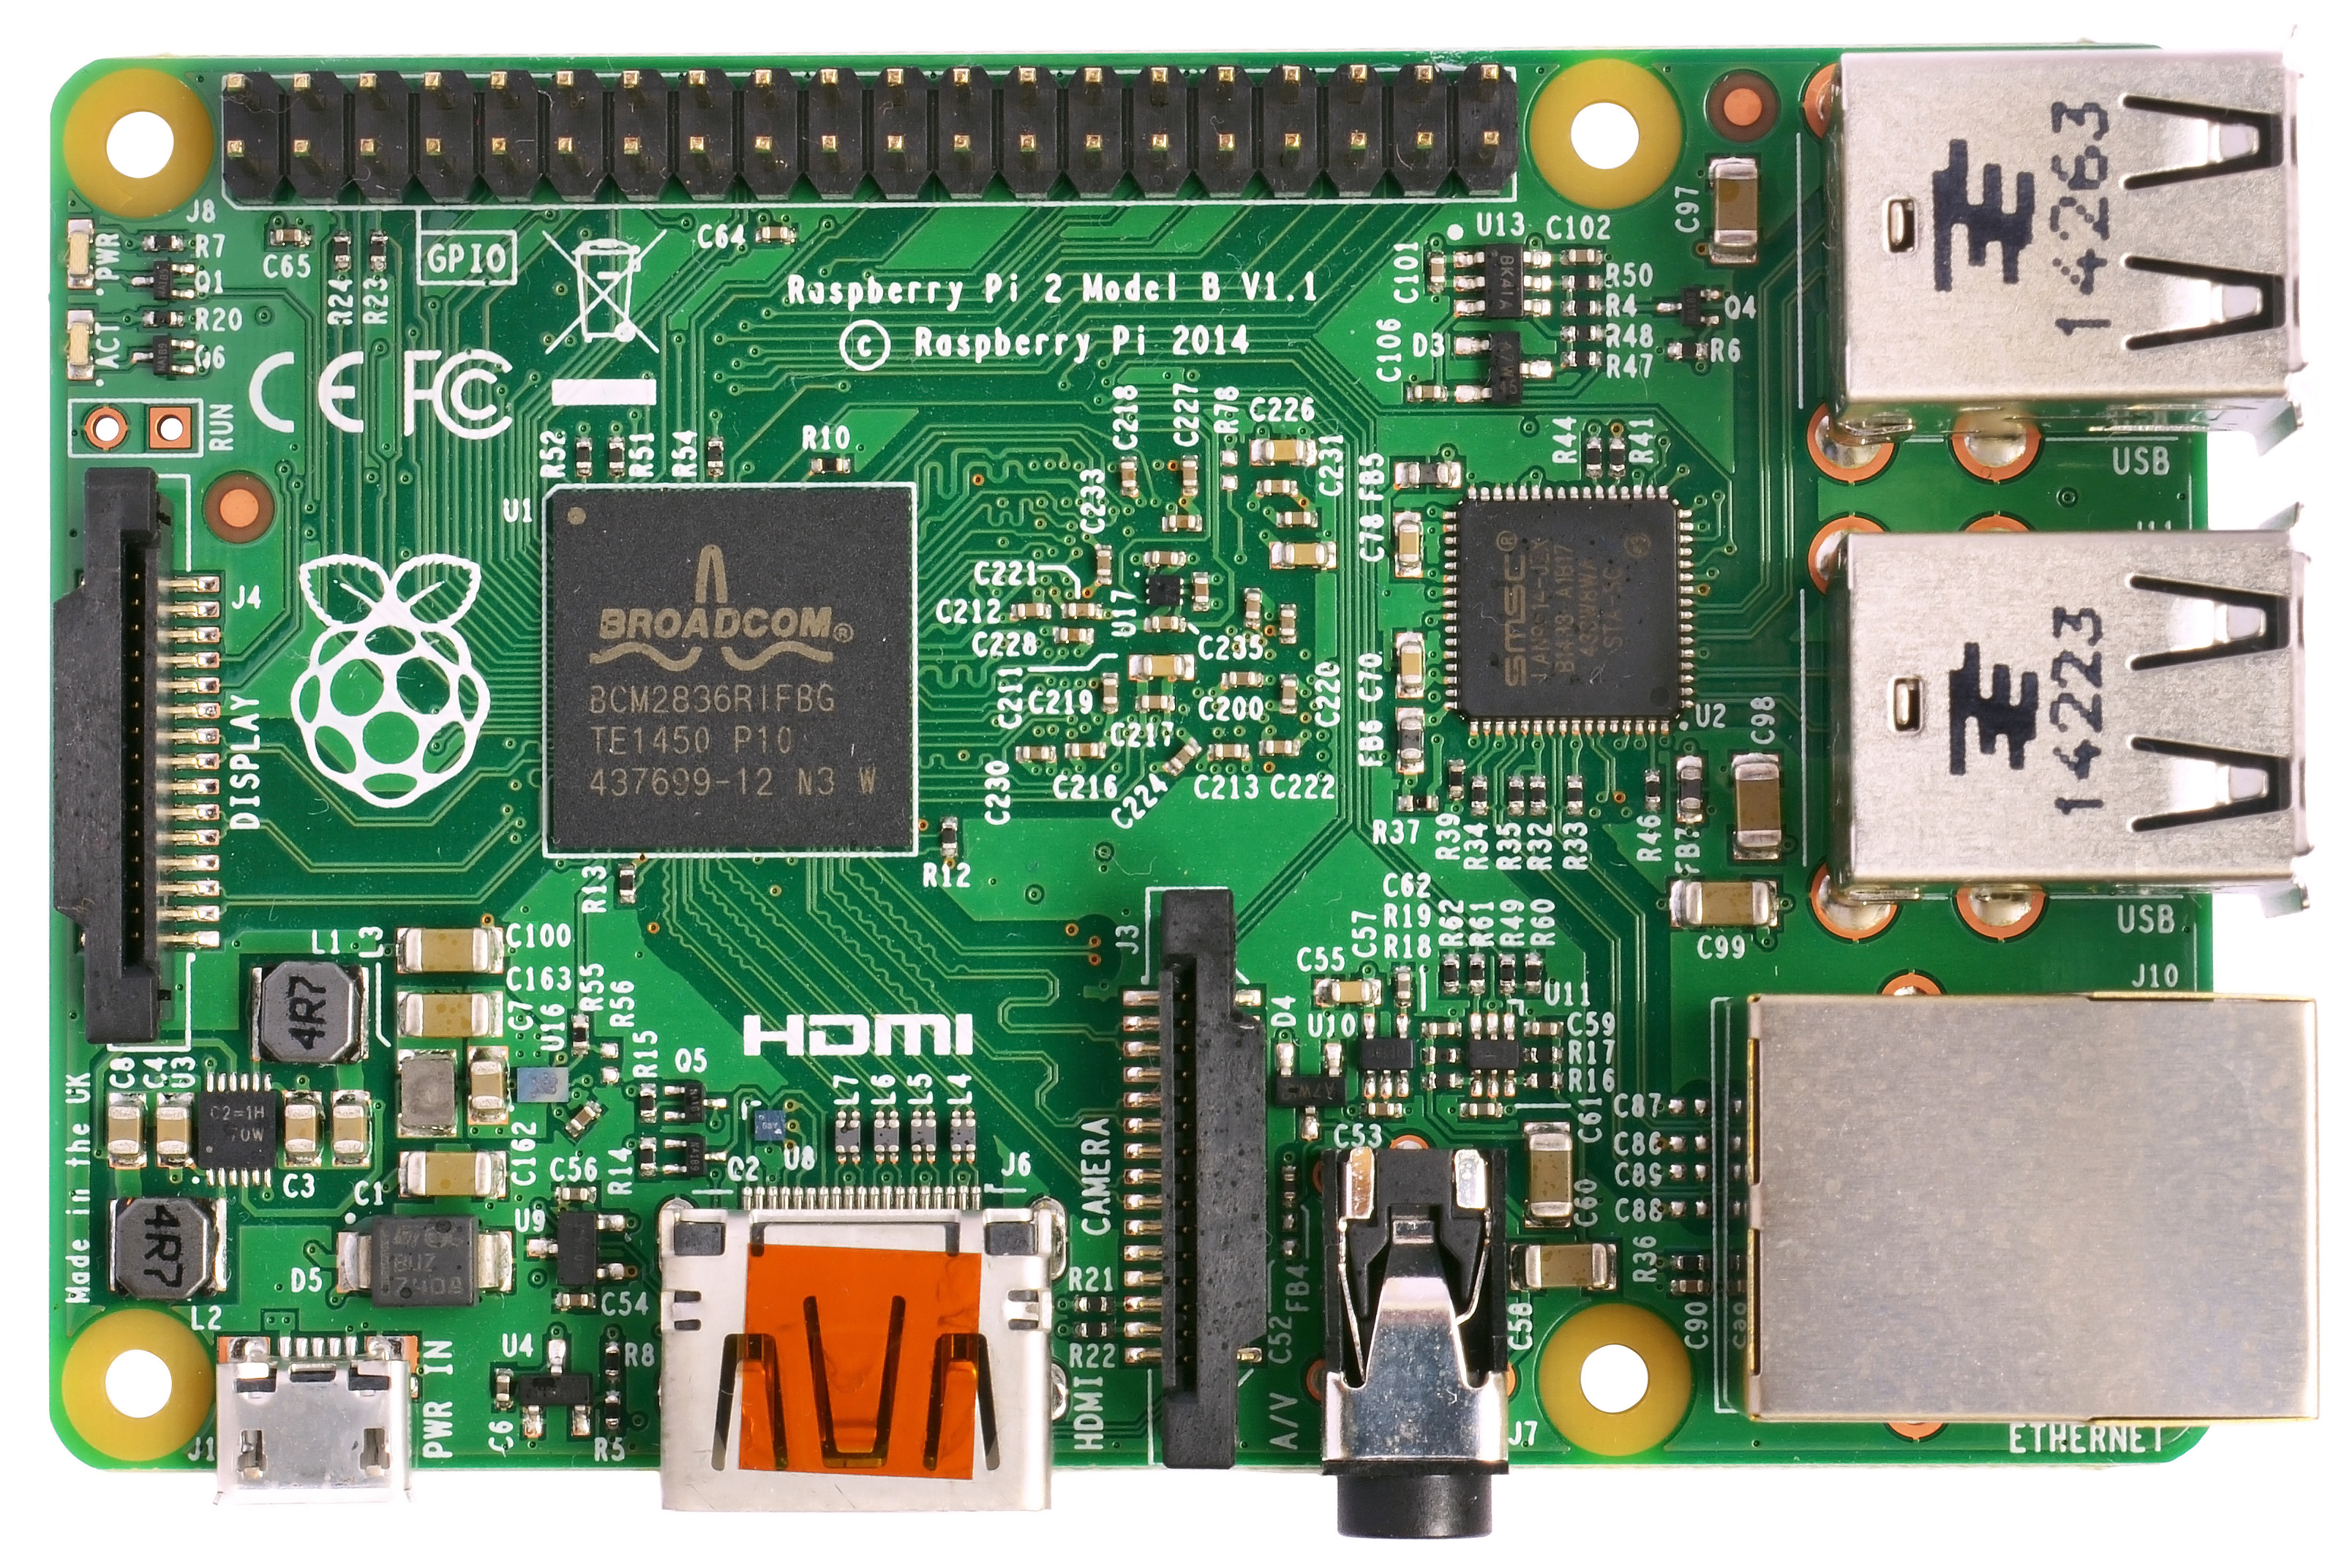
\includegraphics[width=\linewidth]{img/rasp.jpg}
	\label{fig:raspberry}
	\caption[Raspberry Pi w wersji 2 B v1.1]{Raspberry Pi w wersji 2 B v1.1\footnotemark}
\end{figure}
\footnotetext{https://en.wikipedia.org/wiki/Raspberry\_Pi}

Aby obsłużyć technologię RFID użyto modułu z anteną MF RC522 (Rysunek \ref{fig:rfid}). Pracuje on z częstotliwością 13,56 MHz, czyli najpopularniej występującą częstotliwością RFID. Moduł ten łączy się z Raspberry po interfejsie SPI.

\begin{figure}[h!]
	\centering
	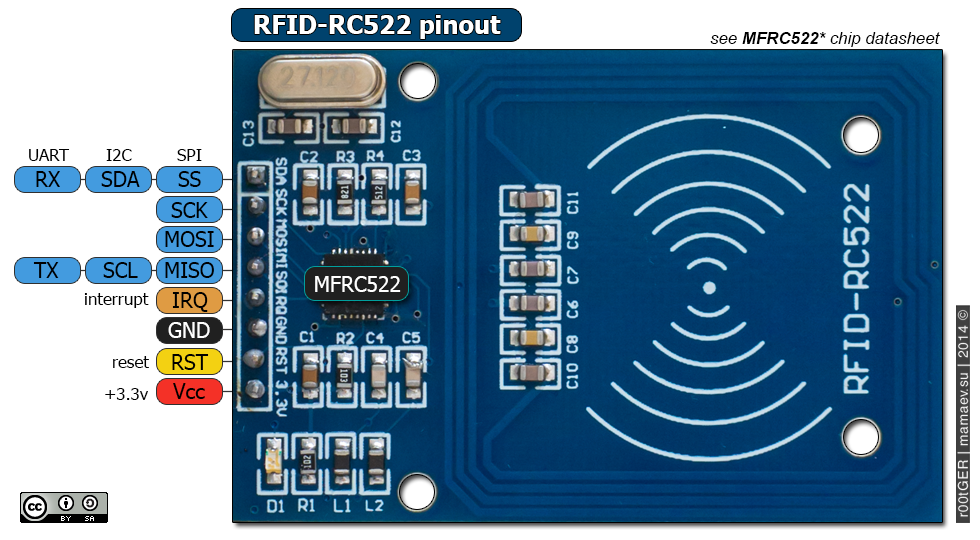
\includegraphics[width=\linewidth]{img/RFID-RC522-pinout.png}
	\label{fig:rfid}
	\caption[Czytnik RFID z anteną MF RC522]{Czytnik RFID z anteną MF RC522\footnotemark}
\end{figure}
\footnotetext{https://github.com/r00tGER/RFID-RC522}

Aby złączyć moduły ze sobą wykorzystana została płytka stykowa, zwana inaczej płytką prototypową (Rysunek \ref{fig:stykowa}).

\begin{figure}[h!]
	\centering
	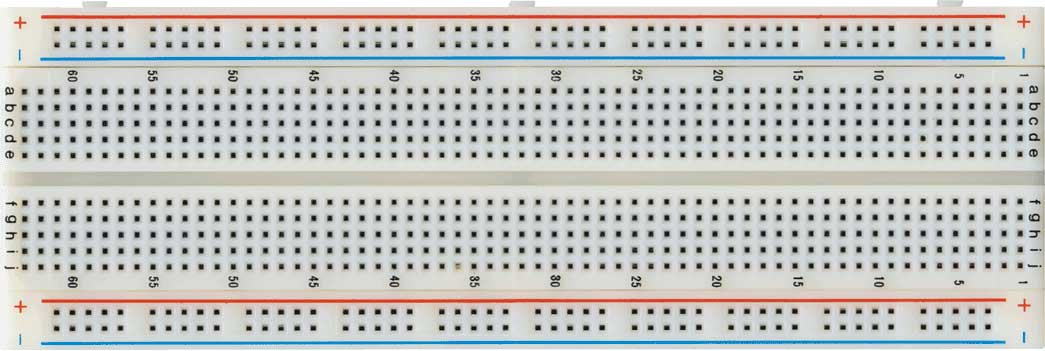
\includegraphics[width=\linewidth]{img/plytka-stykowa.jpg}
	\label{fig:stykowa}
	\caption[Płytka prototypowa na 830 styków]{Płytka prototypowa na 830 styków\footnotemark}
\end{figure}
\footnotetext{http://technovade.pl/arduino/arduino-akcesoria/plytka-stykowa-prototypowa-830-otworow.html}

Do sygnalizacji poprawnej bądź niepoprawnej autoryzacji, użyte zostały dwie zwykłe diody - czerwona do sygnalizacji błędu oraz zielona do sygnalizacji poprawnej autoryzacji. Do połączenia ich z płytką wykorzystano dwa rezystory, o oporności odpowiednio 220 Ohm oraz 150 Ohm.

\section{Podłączenie}

Przed przystąpieniem do realizacji należało najpierw przylutować czytnik RFID do goldpinów, gdyż w przeciwnym wypadku siła sygnału byłaby za słaba, aby móc przesyłać dane do oraz z powrotem z płytki. Po zlutowaniu podłączono wszystkie styki czytnika do pinów SPI, zgodnie z dokumentacją modułu MFRC522 (Pozycja \cite{mfrc}) oraz schematem rozłożenia wyjść na płytce (Pozycja \cite{piny}).

MFRC522 podłączony został do poniższych portów (pin IRQ nie jest wymagany do podłączenia, więc pozostał luźny):

\begin{table}[h!]
\centering
\caption{Połączenia pinów czytnika RFID}
\label{piny}
\begin{tabular}{@{}|c|c|c|@{}}
\toprule
\textbf{MFRC522} & \textbf{Numer pinu Raspberry} & \textbf{Nazwa pinu} \\ \midrule
SDA & 24 & GPIO8 \\ \midrule
SCK & 23 & GPIO11 \\ \midrule
MOSI & 19 & GPIO10 \\ \midrule
MISO & 21 & GPIO9 \\ \midrule
IRQ & x & x \\ \midrule
GND & 9 & GND \\ \midrule
RST & 22 & GPIO25 \\ \midrule
3.3V & 1 & 3V3 \\ \bottomrule
\end{tabular}
\end{table}

Diody podłączone zostały jak na Rysunku \ref{fig:led}, czyli katodę diody czerwonej podłączono do masy, zaś anodę poprzez 220-Ohmowy rezystor do pinu GPIO24. Dioda zielona podłączona została bardzo podobnie, z tą różnicą, że spięto ją z pinem GPIO23 oraz ze względu na większe natężenie prądu potrzebne do jej zaświecenia, zastosowano opornik 150-Ohmowy.

\begin{figure}[h!]
	\centering
	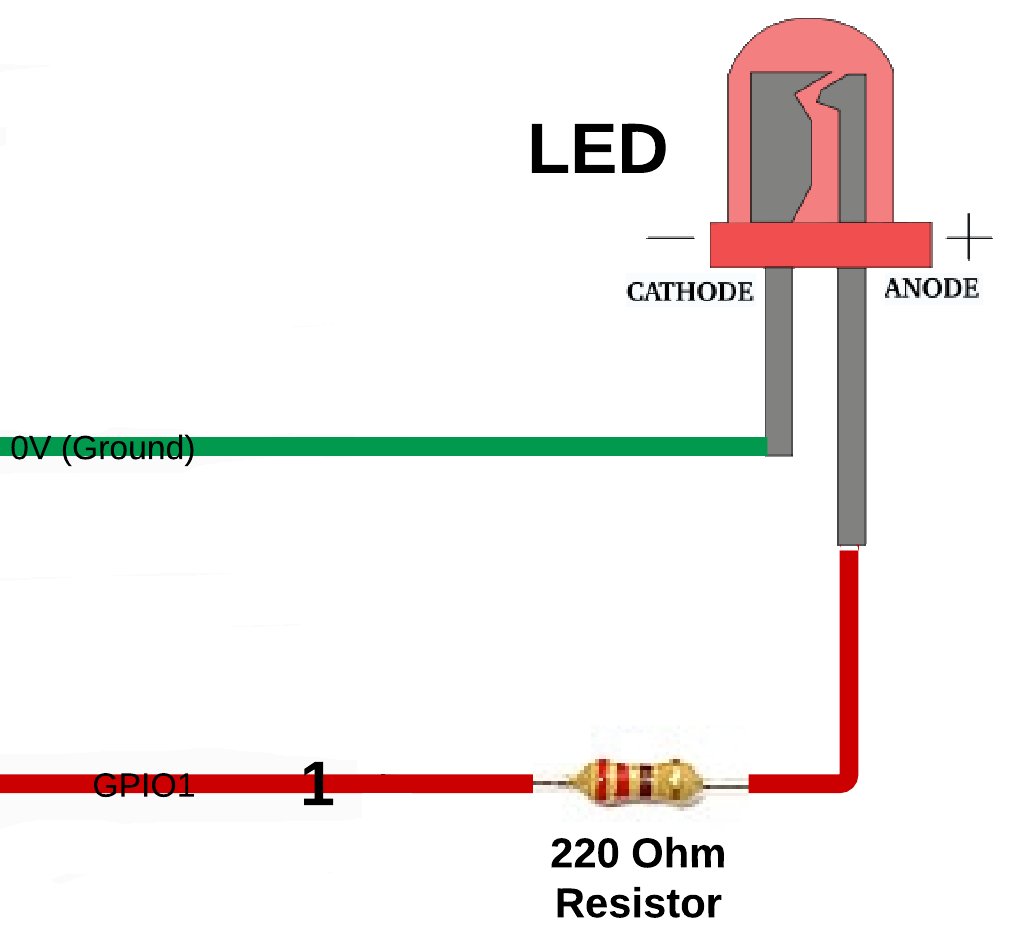
\includegraphics[width=0.5\linewidth]{img/led.png}
	\label{fig:led}
	\caption[Podłączenie czerwonej diody]{Podłączenie czerwonej diody}
\end{figure}

\newpage

Poniższy schemat z programu Fritzing\footnote{http://fritzing.org/home/} przedstawia finalny układ połączeń.

\begin{figure}[h!]
	\centering
	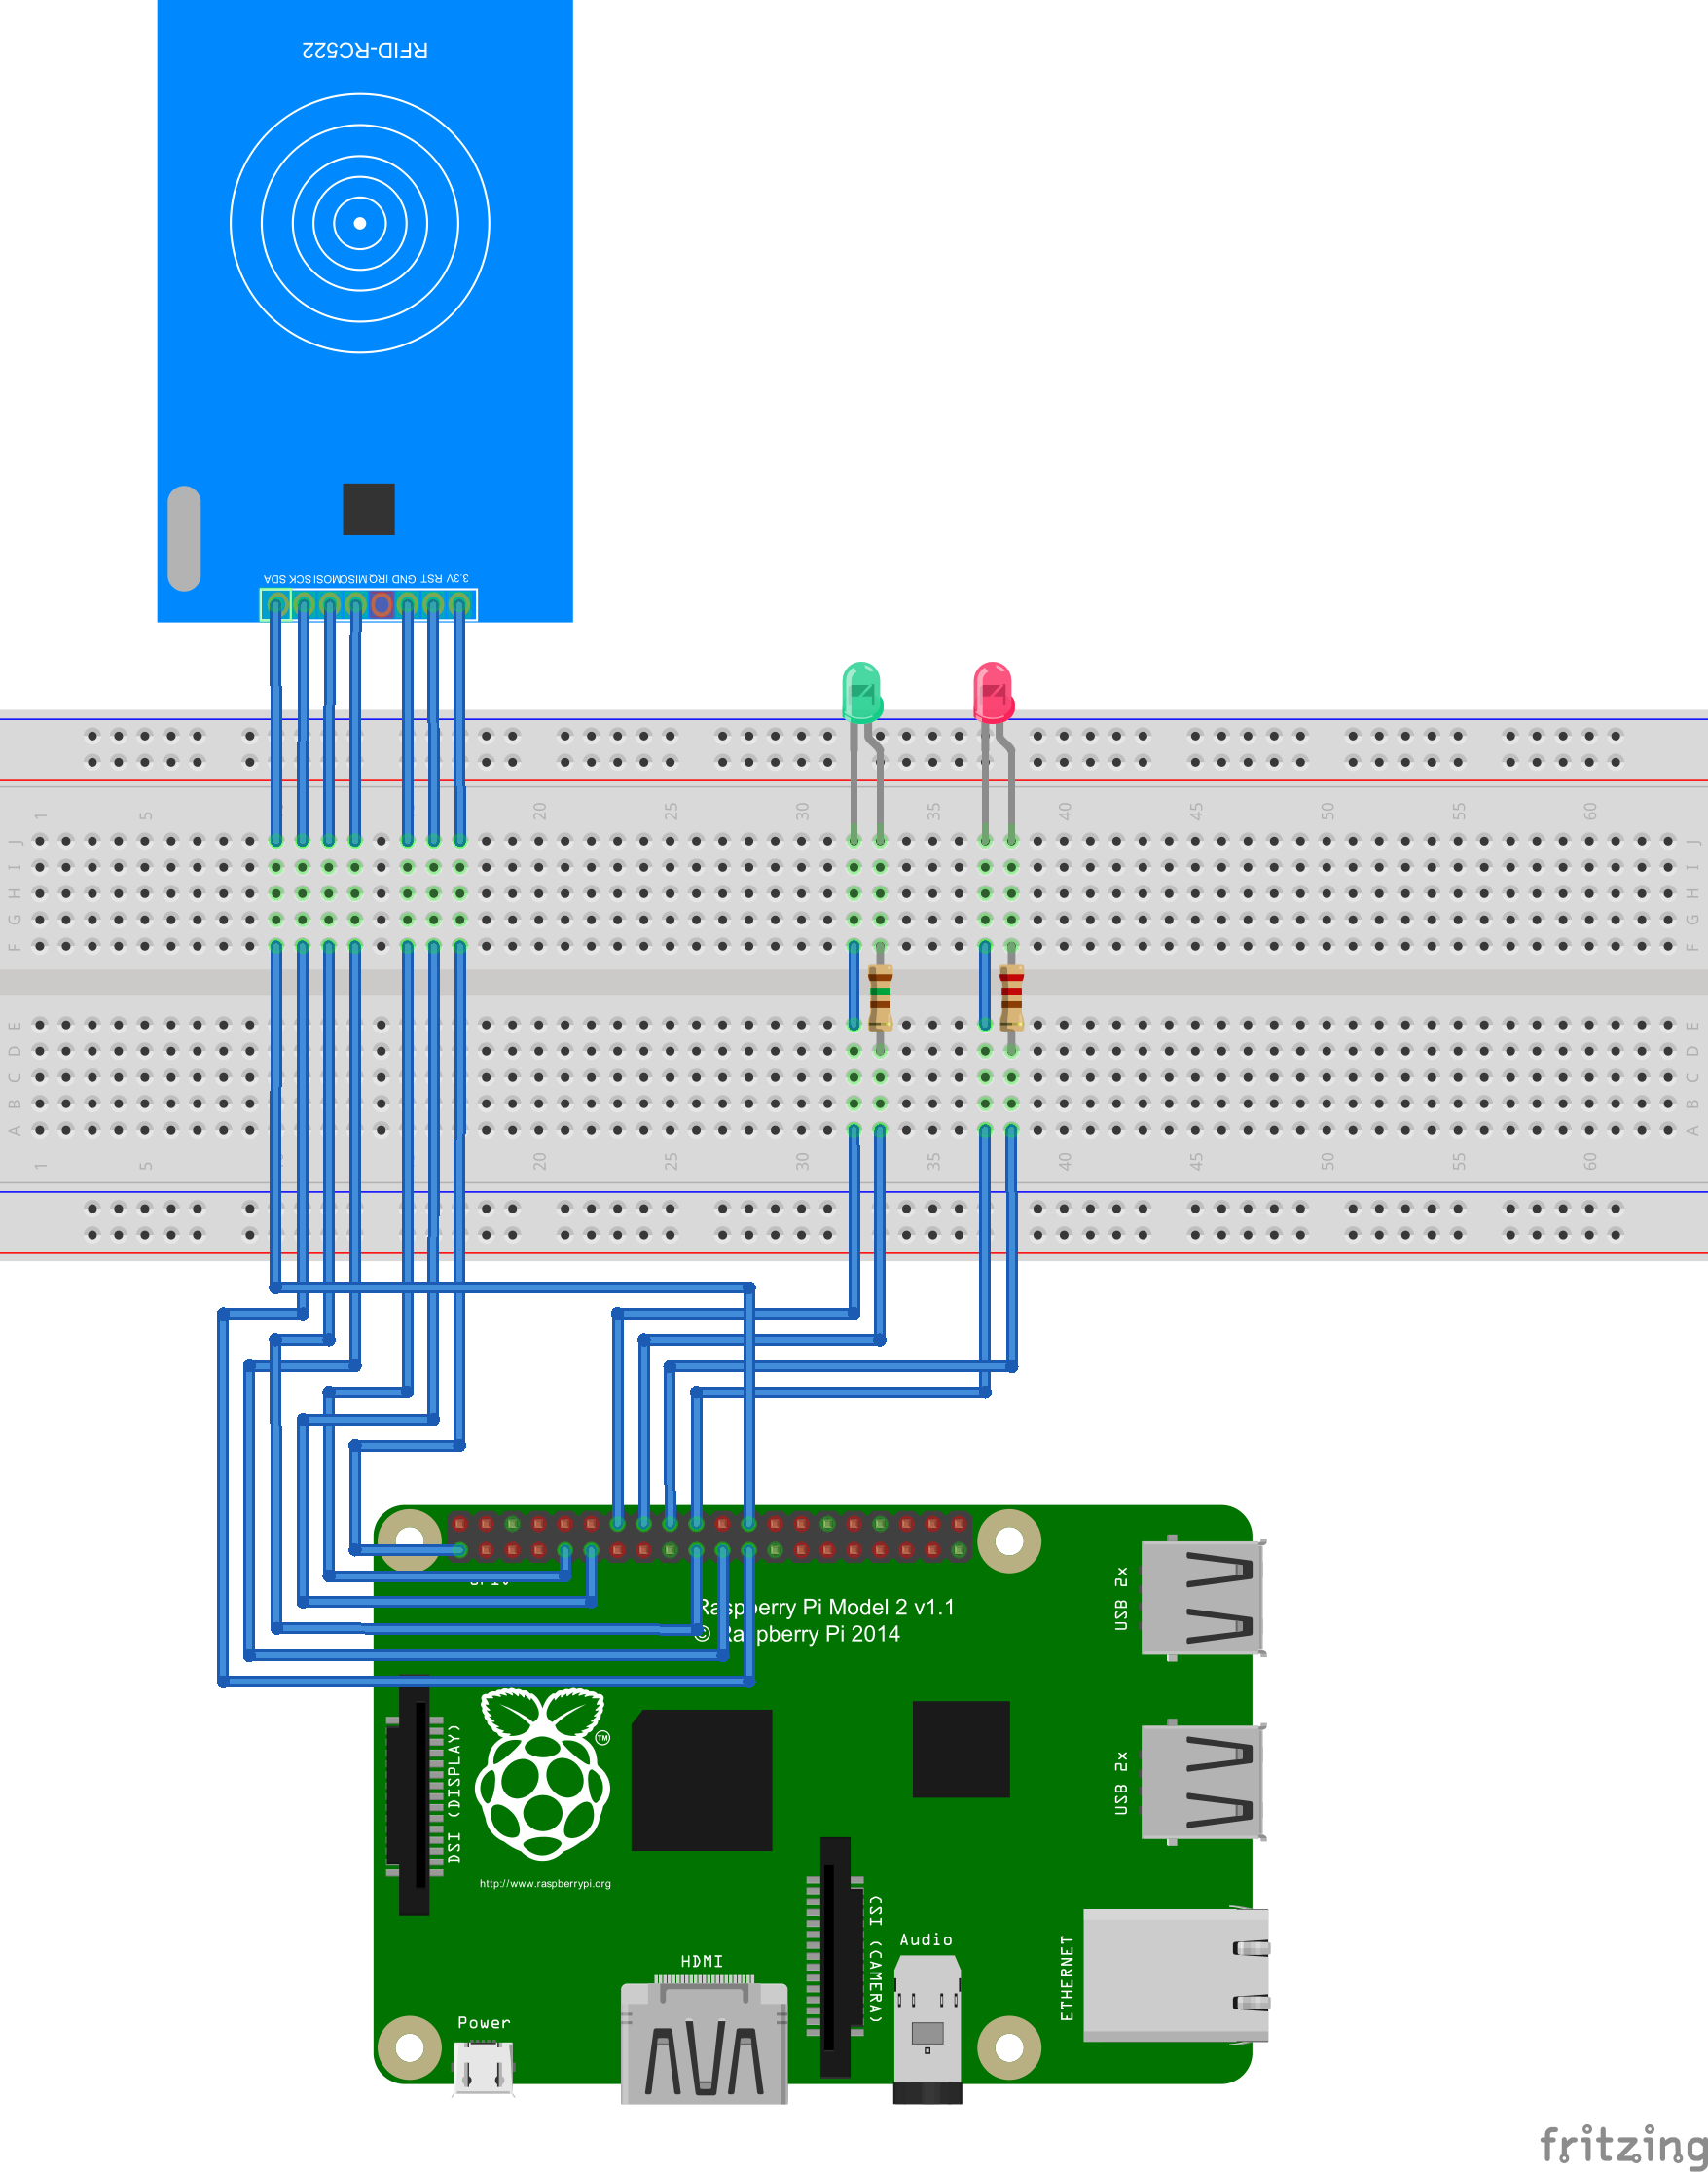
\includegraphics[width=\linewidth]{img/projekt_bb.png}
	\label{fig:projekt}
	\caption[Finalny wygląd połączeń]{Finalny wygląd połączeń}
\end{figure}

\section{Konfiguracja}

Aby zmusić kod do działania, należy skonfigurować potrzebne narzędzia i biblioteki. Należy najpierw uruchomić do działania porty SPI. Aby tego dokonać wpisujemy w terminalu:

\begin{verbatim}
$ sudo raspi-config
\end{verbatim}

Następnie przejść do Advanced Options i przestawić SPI na Enabled. Na starszych wersjach Raspberry należało również SPI z listy zablokowanych, poprzez uruchomienie edytora:

\begin{verbatim}
$ sudo nano /etc/modprobe.d/raspi-blacklist.conf
\end{verbatim}

I zakomentowanie linii dodając przed nią znak \#:

\begin{verbatim}
blacklist spi-bcm2708
\end{verbatim}

Kolejnym krokiem jest zrestartowanie urządzenia, i po restarcie wpisanie:

\begin{verbatim}
$ ls /dev/spidev0.*
\end{verbatim}

Powinniśmy otrzymać wynik podobny do następującego, co świadczy o tym, że SPI zostało uruchomione poprawnie:

\begin{verbatim}
/dev/spidev0.0 /dev/spidev0.1
\end{verbatim}

Kolejnym krokiem jest włączenie drzewa urządzeń. Należy wpisać:

\begin{verbatim}
$ sudo nano /boot/config.txt
\end{verbatim}

I dodać na końcu pliku następującą linijkę:

\begin{verbatim}
device_tree=on
\end{verbatim}

Następnie należy jeszcze zaktualizować sterownik dla mikrokontrolera Broadcom BCM 2835. Pobieramy jego najnowszą wersję \footnote{http://www.airspayce.com/mikem/bcm2835/} i wpisujemy kolejno:

\begin{verbatim}
$ tar zxvf bcm2835-1.xx.tar.gz
$ cd bcm2835-1.xx
$ ./configure
$ make
$ sudo make check
$ sudo make install
\end{verbatim}

Po tych krokach urządzenie jest już skonfigurowane do korzystania z SPI oraz modułu RFID.

\newpage

\section{Oprogramowanie}

Oprogramowanie napisane zostało w języku Python i wykorzystuje do działania dwie zewnętrzne biblioteki. Pierwszą jest SPI-Py\footnote{https://github.com/lthiery/SPI-Py}, która umożliwia korzystanie z interfejsu SPI z poziomu interpretera Python. Drugą jest MFRC522-python\footnote{https://github.com/mxgxw/MFRC522-python}, dzięki której można korzystać z modułu czytnika kart RFID.

W aplikacji wyróżnić można kilka modułów:

\begin{enumerate}
  \item \texttt{main.py} - główny moduł systemu, odpowiada za pętlę programu.
  \item \texttt{logger.py} - moduł odpowiedzialny za obsługę logów aplikacji.
  \item \texttt{database.py} - łączenie się z bazą danych oraz dodawanie do niej rekordów.
  \item \texttt{nfc.py} - obsługa odczytywania danych z karty.
\end{enumerate}

Program uruchamia się wpisując w konsoli (wymagana jest wersja Pythona co najmniej 3.0):

\begin{verbatim}
python3 main.py
\end{verbatim}

Aplikacja spróbuje teraz połączyć się z bazą danych i w wypadku pomyślnego połączenia uruchomiona zostanie główna pętla programu. Pętla ta uruchamia mniejszą pętlę w module \texttt{nfc.py}, który to w czasie ciągłym (aż do momentu wciśnięcia kombinacji klawiszy Ctrl + C) uruchamia cewkę na module MFRC522 i sprawdza czy w pobliżu nie znajduje się karta RFID. Jeśli tak, to odczytywany jest identyfikator karty, który następnie porównywany jest z identyfikatorami wszystkich przypisanych do systemu użytkownikami. Jeśli Id zostanie odnaleziony, do bazy zostaje dodany pod Id pracownika timestamp z aktualną datą i godziną odbicia się. System sygnalizuje też poprawną autoryzację miganiem zielonej diody. Jeśli identyfikator nie zostanie odnaleziony w bazie, system sygnalizuje to miganiem diody czerwonej.

Aplikacja kończy swe działanie w momencie wykrycia kombinacji klawiszy Ctrl + C, kończąc działanie modułu MFRC522 i zamykając połączenie do bazy danych.